% !TEX root = ../5.DISTILLATION.tex
\section{EXPERIMENTAL THEORY}

The separation dynamics are most heavily dependent on the vapor pressure of the species in the column. The more volatile component is also known as the light key, the less volatile component is also known as the heavy key. For a two-component separation:

\begin{equation}
    \alpha = \frac{K_L}{K_H}
\end{equation}

\begin{equation}
    K_L = \frac{P_L}{P}
\end{equation}

\begin{equation}
    K_H = \frac{P_H}{P}
\end{equation}

All symbols are defined in the nomenclature section at the end of the text. By Raoult's law, this means that relative volatility can be described in terms of mole fractions in the liquid and vapor phases.

\begin{equation}
    \alpha = \frac{y_L/x_L}{y_H/x_H} = \frac{y_L(1 - x_L)}{x_L(1 - y_L)}
\end{equation}

This can be rearranged to give:

\begin{equation}
    y_L = \frac{\alpha x_L}{1 + x_L(\alpha - 1)}
\end{equation}

The traditional approach to modeling distillation processes is known as the McCabe-Thiele approach. This model requires making the following assumptions:
\begin{itemize}
    \item That the relative volatility is constant over the temperature range in the column.
    \item That the components have equal and constant molar enthalpy.
    \item That enthalpy changes and heat of mixing are negligible.
    \item That the pressure is uniform within the column.
\end{itemize}

These assumptions allow equations to be derived relating flow rates to molar compositions in each stage of the column. The column is divided into the vapor phase, and the rectification section, in which the less volatile component is selectively condensed. In each section, the liquid and vapor compositions can be related to flow rates.

\textbf{Rectification section:}
\begin{equation}
    V_{n+1}y_{n+1} = L_n x_n + D x_D
\end{equation}
\begin{equation}
    y_{n+1} = \frac{L_n}{V_{n+1}}x_n + \frac{D}{V_{n+1}}x_D
\end{equation}
where the stages are numbered consecutively, beginning with the top stage.
\begin{equation}
    \frac{L}{V} = \frac{R}{R+1}
\end{equation}
\begin{equation}
    y_n = \frac{R}{R+1}x_n + \frac{1}{R+1}x_D
\end{equation}

\textbf{Stripping section:}
\begin{equation}
    y_n = \frac{L_n}{V_n}x_n - \frac{B}{V_n}x_B
\end{equation}
\begin{equation}
    V_B = \frac{V}{B}
\end{equation}
\begin{equation}
    \frac{L}{V} = \frac{V+B}{V} = \frac{V_B+1}{V_B}
\end{equation}
\begin{equation}
    y_n = \frac{V_B+1}{V_B}x_n - \frac{1}{V_B}x_B
\end{equation}

Given equilibrium data for the components of the distillation, these equations can be used to model the stages graphically, as shown in Figure \ref{fig:mccabe_thiele}.

\begin{figure}[H]
    \centering
    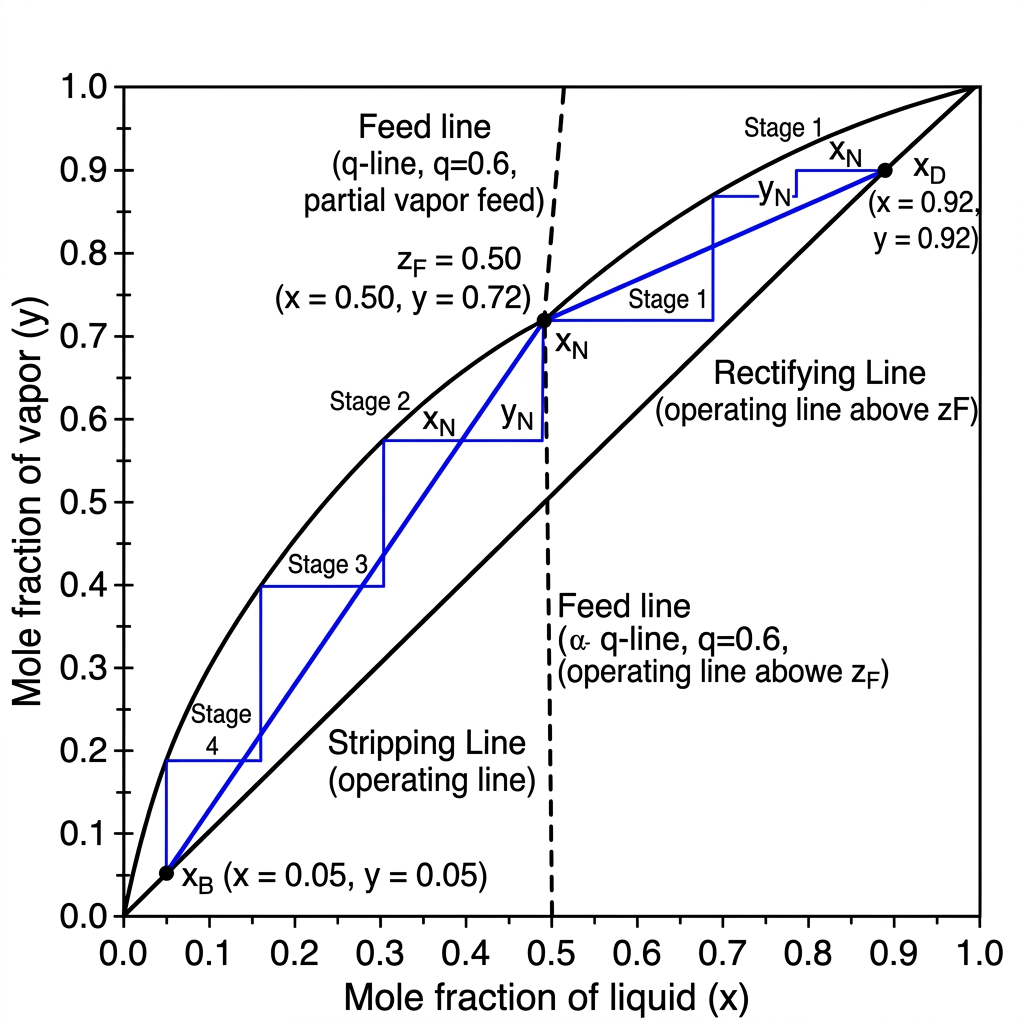
\includegraphics[width=0.6\textwidth]{Images/mccabe_thiele.png}
    \caption{Sample McCabe-Thiele diagram. Each step indicates a theoretical stage going to complete equilibrium. The calculations are shown for the rectification section only.}
    \label{fig:mccabe_thiele}
\end{figure}

Because true vapor-liquid equilibrium is unlikely to be achieved on each stage, this method must be adapted in order to properly model the distillation system. A widely used method for this is known as Murphree Efficiency:
\begin{equation}
    E_M = \frac{y_n - y_{n+1}}{y_n^* - y_{n+1}}
\end{equation}

Where $y^*$ used in this equation is derived from experimentally measured liquid-phase composition values. The Murphree Efficiency can be used to alter the equilibrium line in the McCabe-Thiele graph. This adapted graph can be used to more accurately predict the separation under different conditions of feed composition and reflux ratios.
